\newpage
%%%%%%%%%%%%%%%%%%%%  解答（旧 prob_p72_2.png〜prob_p76_1.png）  %%%%%%%%%%%%%%%%%%%%
\setlength{\columnseprule}{0.4pt}
\begin{multicols}{2}
\raggedcolumns

{\gtfamily\large 第3回　物体に作用する力とつり合い}\par\vspace{2mm}

\Rank{A問題}
\MonN{19}{基本事項の確認}\par\nopagebreak
\begin{sisin}
\hspace{1zw}物体に作用する力は，場の力，接触力，作用・反作用の順番に考えていくとよい．なお，場の力である重力は，地球が物体を引く力であるから作用主は地球である．
\end{sisin}
\noindent{\gtfamily 【解答】}\par\nopagebreak
\begin{zuright}{24mm}
\begin{komon}
\ko{1} 重力$W$\\
ばねが物体に及ぼす弾性力$F$
\end{komon}
\zusep
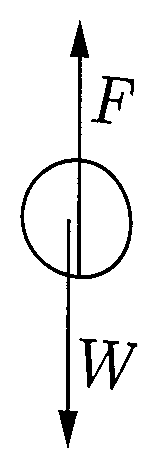
\includegraphics[keepaspectratio,height=26mm]{fig/ch3_p72_19a.png}
\end{zuright}
\begin{zuright}{28mm}
\begin{komon}
\ko{2} 重力$W$\\
右の糸が物体に及ぼす張力$T_1$\\
左の糸が物体に及ぼす張力$T_2$
\end{komon}
\zusep
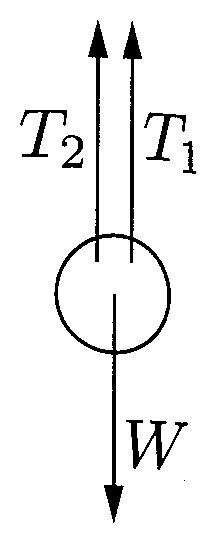
\includegraphics[keepaspectratio,height=30mm]{fig/ch3_p72_19b.png}
\end{zuright}
\begin{zuright}{32mm}
\begin{komon}
\ko{3} 重力$W$\\
右の斜面が物体に及ぼす垂直抗力$N_1$\\
左の斜面が物体に及ぼす垂直抗力$N_2$
\end{komon}
\zusep
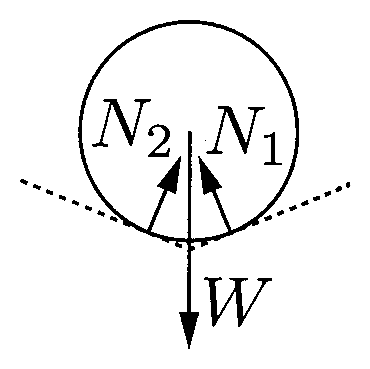
\includegraphics[keepaspectratio,width=28mm]{fig/ch3_p72_19c.png}
\end{zuright}

\MonN{20}{基本事項の確認}\par\nopagebreak
\begin{sisin}
\hspace{1zw}力のつり合いと，作用・反作用の関係とは異なるものであることに注意せよ．力のつり合いとは，\underline{ある一つ}\hskip0pt\underline{の物体に}\hskip0pt\underline{作用する}\hskip0pt\underline{いくつか}\hskip0pt\underline{の力が}\hskip0pt\underline{互いに}\hskip0pt\underline{打ち消し}\hskip0pt\underline{合っている}ことを言い，作用・反作用の関係とは，\underline{二つの}\hskip0pt\underline{物体が}\hskip0pt\underline{互いに}\hskip0pt\underline{及ぼし}\hskip0pt\underline{合っている}\hskip0pt\underline{等大・}\hskip0pt\underline{逆向きの力}のことを言う．単純に大きさだけを見て，これが同じだからつり合いとしたり，作用・反作用であるとはしないこと．また，接触力は互いに接触していなければ作用しないので，\MARU{7}の力は存在しない．

\hspace{1zw}存在する力を「$\mathrm{A}$が$\mathrm{B}$に及ぼす○○力」と正しく言って考えると分かりやすい．つりあいの関係になるのは，「$\mathrm{B}$に」の部分が共通する複数の力である．また，作用・反作用の関係になる力は「$\mathrm{A}$が$\mathrm{B}$に」の部分が「$\mathrm{B}$が$\mathrm{A}$に」となる一組の力である．
\end{sisin}
\noindent{\gtfamily 【解答】}\par\nopagebreak
\hspace{1zw}力の作用図は次図のようになる．
\begin{center}
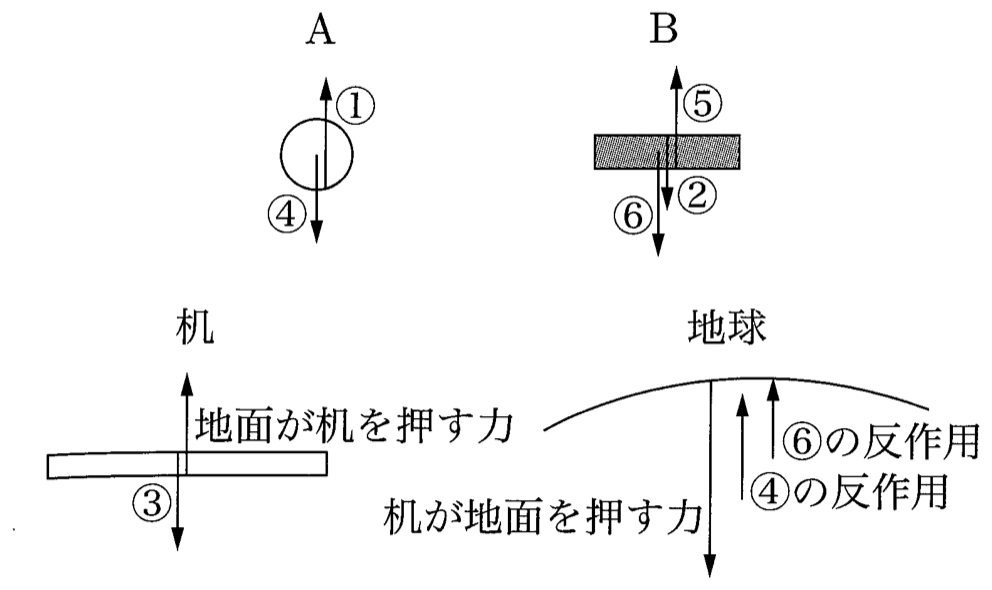
\includegraphics[keepaspectratio,width=70mm]{fig/ch3_p73_20.png}
\end{center}
\begin{komon}
\ko{1} つり合いの関係

物体$\mathrm{A}$に関して，鉛直下向きに作用する\MARU{4}と鉛直上向きに作用する\MARU{1}の力がつり合う．

板$\mathrm{B}$に関して，鉛直下向きに作用する\MARU{2}＋\MARU{6}と鉛直上向きに作用する\MARU{5}の力がつり合う．
\ko{2} 作用・反作用の関係

$\mathrm{A}$と$\mathrm{B}$間でやり取りされる垂直抗力\MARU{1}と\MARU{2}が，また$\mathrm{B}$と机間でやり取りされる垂直抗力\MARU{3}と\MARU{5}とが互いに作用・反作用の関係にある．
\end{komon}

\Rank{B問題}
\MonN{21}{力のつり合い}\par\nopagebreak
\begin{sisin}
\hspace{1zw}まず，物体に作用する力を，場の力，接触力，作用・反作用の力の順に描き出す．物体が静止している場合には描き出した力の作用図をもとにつり合い条件を考えればよい．

\hspace{1zw}力のつり合い条件のとらえ方はベクトル的に考える方法，成分分解する方法とがあるが，本問の場合は糸が2本あり，ある特殊な方向というのは考えにくい．そこで，オーソドックスに水平方向・鉛直方向に力を成分分解して，各軸方向の力のつり合いを考える．
\end{sisin}
\noindent{\gtfamily 【解答】}\par\nopagebreak
\hspace{1zw}物体に働く力の作用図は次図の通り．
\begin{center}
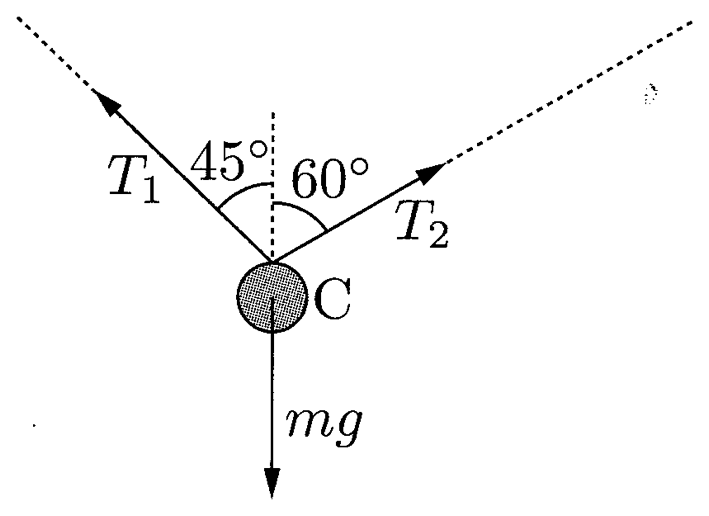
\includegraphics[keepaspectratio,width=50mm]{fig/ch3_p73_21.png}
\end{center}
\hspace{1zw}鉛直方向・水平方向のつり合いの式は，
\[
\text{鉛直方向：}\quad T_1\cos45^\circ+T_2\cos60^\circ=mg
\]
\[
\text{水平方向：}\quad T_1\sin45^\circ=T_2\sin60^\circ
\]
以上2式より，
\[
T_1=\dfrac{\sqrt2}{2}\left(3-\sqrt3\right)mg\U{N}
\]
\[
T_2=\left(\sqrt3-1\right)mg\U{N}\Ans
\]

\MonN{22}{弾性力}\par\nopagebreak
\begin{sisin}
\hspace{1zw}まず作用している力を書き出す必要がある．\underline{どの}\hskip0pt\underline{物体}\hskip0pt\underline{に対}\hskip0pt\underline{して}\hskip0pt\underline{力が}\hskip0pt\underline{作用}\hskip0pt\underline{する}\hskip0pt\underline{かに}\hskip0pt\underline{注意}\hskip0pt\underline{せよ}．物体$\mathrm{A}$については場の力として重力$m_1g$，接触力としてバネから弾性力$kx$，糸から張力$T$を受けるが，物体$\mathrm{B}$については場の力として重力$m_2g$と接触力の張力$T$の\underline{二つのみ}である．物体$\mathrm{B}$には糸しか接触しておらず，バネは接触していないから弾性力$kx$は$\mathrm{B}$には作用しない．

\hspace{1zw}同様に，各物体に対しての力のつり合いを考える際には，\underline{他の物体}\hskip0pt\underline{に作用する}\hskip0pt\underline{力を含め}\hskip0pt\underline{ては}\hskip0pt\underline{ならない}．すなわち，$\mathrm{B}$に関する力のつり合いを考えるときに$\mathrm{A}$に作用する弾性力$kx$を考えてはならないし，また$\mathrm{A}$に関する力のつり合いを考えるときに$\mathrm{B}$に作用する重力$m_2g$を含めてはならない．
\end{sisin}
\noindent{\gtfamily 【解答】}\par\nopagebreak
\begin{komon}
\ko{1} ばねののびを$x\U{m}$，糸の張力の大きさを$T\U{N}$とする．$\mathrm{A}$，$\mathrm{B}$に作用する力の作用図は次図の通りとなる．
\begin{center}
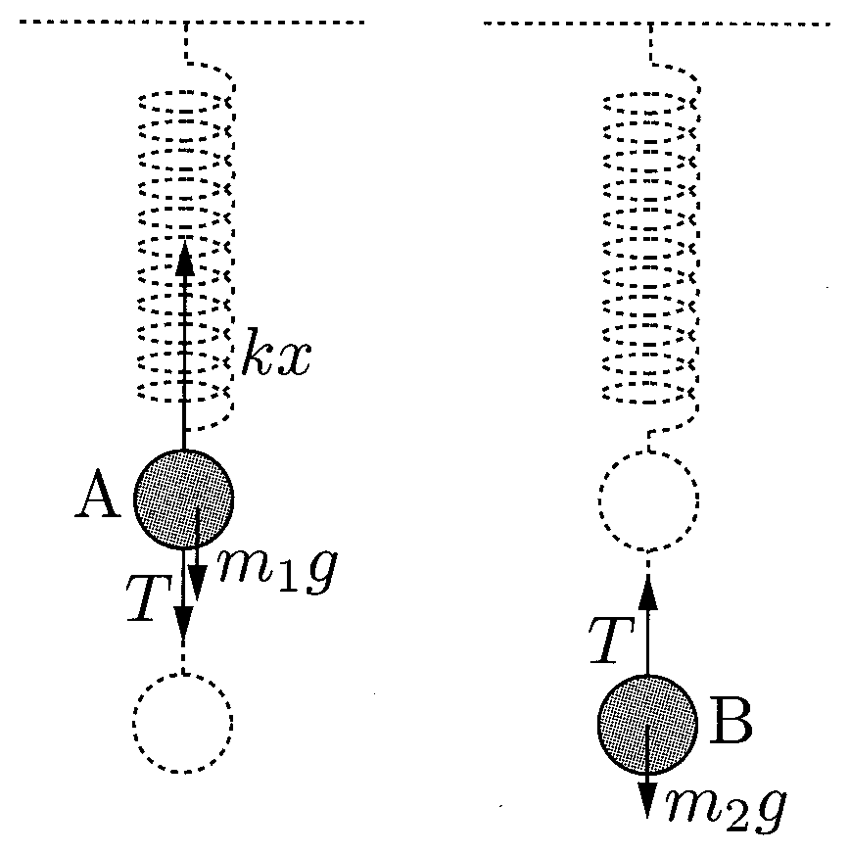
\includegraphics[keepaspectratio,width=60mm]{fig/ch3_p73_22.png}
\end{center}

よって，各物体の鉛直方向の力のつり合いの式は，
\[
\mathrm{A}:kx=m_1g+T
\]
\[
\mathrm{B}:T=m_2g
\]
以上2式より，
\[
T=m_2g\U{N}\Ans
\]
\ko{2} また，$x$については，
\[
x=\dfrac{(m_1+m_2)g}{k}\U{m}\Ans
\]
\end{komon}

\MonN{23}{斜面上での最大摩擦力}\par\nopagebreak
\begin{sisin}
\hbadness=10000
\hspace{1zw}まず，各物体に作用する力を書き出して力のつり合い条件を考えよ．\underline{静止}\hskip0pt\underline{摩擦}\hskip0pt\underline{力お}\hskip0pt\underline{よび}\hskip0pt\underline{垂直}\hskip0pt\underline{抗力}\hskip0pt\underline{の大}\hskip0pt\underline{きさ}\hskip0pt\underline{は力}\hskip0pt\underline{のつ}\hskip0pt\underline{り合}\hskip0pt\underline{いの}\hskip0pt\underline{条件}\hskip0pt\underline{式か}\hskip0pt\underline{ら決}\hskip0pt\underline{まる}ことに注意．静止摩擦力の大きさは$\mu_0N$とは限らない．本問のように，滑り出すギリギリのときには作用する静止摩擦力は最大摩擦力$\mu_0N$となるが，最初から$\mu_0N$とはおかずに，まず静止摩擦力を$f$とおき，つり合いの条件から$f$を求めて考えること．

\hspace{1zw}また，斜面上の物体のつり合いは斜面に対して平行な方向とそれに垂直な方向に力を分解して考える．
\end{sisin}
\noindent{\gtfamily 【解答】}\par\nopagebreak
\hspace{1zw}板が物体に及ぼす垂直抗力の大きさを$N\U{N}$，静止摩擦力の大きさを$f\U{N}$とする．また物体と面との間の静止摩擦係数を$\mu_0$とする．
\begin{komon}
\ko{1} 水平方向に加える外力の大きさを$F\U{N}$とするとき，物体をつり合わせるために静止摩擦力はこの外力と逆向きに作用する．ゆえに，このとき物体に働く力の作用図は次図の通り．
\begin{center}
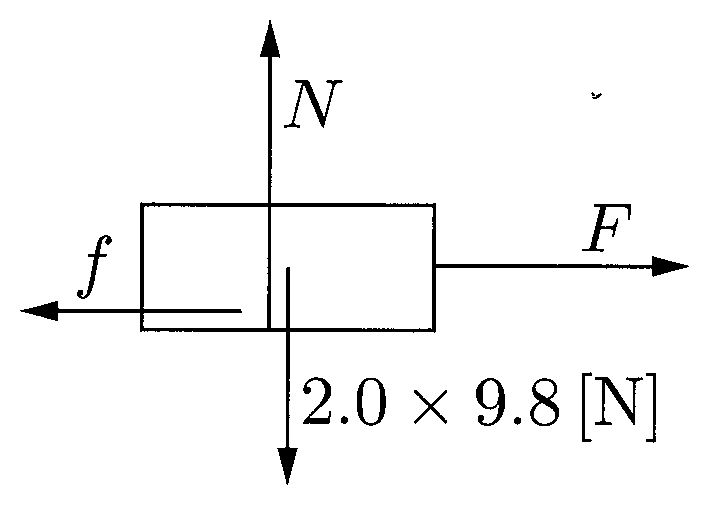
\includegraphics[keepaspectratio,width=55mm]{fig/ch3_p74_23a.png}
\end{center}

ここで，力のつり合いの条件より，
\[
\text{水平方向：}\quad f=F
\]
\[
\text{鉛直方向：}\quad N=2.0\times9.8\U{N}
\]
静止摩擦力の性質より，$f>\mu_0N=\mu_0\cdot19.6\U{N}$となると物体は滑り出すが，滑り出す瞬間の外力$F$が$8.0\U{N}$であったことから，
\[
8.0=\mu_0\cdot19.6\U{N}
\]
が成立する．よって，静止摩擦係数は
\[
\mu_0=0.408\fallingdotseq0.41\Ans
\]
\ko{2} 斜面の傾斜角が$\varphi$のときについて考える．重力の斜面方向分力$mg\sin\varphi=19.6\sin\varphi$が斜面に沿って下向きに作用して物体を滑らせようとするので，物体に作用する静止摩擦力は斜面に沿って上向きである．よって，物体に作用する力は次図の通り．
\begin{center}
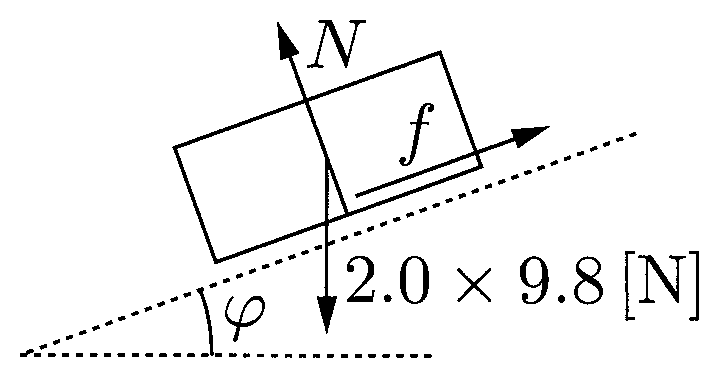
\includegraphics[keepaspectratio,width=55mm]{fig/ch3_p74_23b.png}
\end{center}

ここで，力のつり合いの条件より，
\[
\text{斜面に平行：}\quad 2\times9.8\sin\varphi=f
\]
\[
\text{斜面に垂直：}\quad N=2\times9.8\cos\varphi
\]
ゆえに，
\[
f=19.6\sin\varphi\U{N}
\]
となるが，傾斜角$\varphi$を増していくと静止しつづけるために必要な静止摩擦力は増加していき，
\[
f=\mu_0N
\]
となった直後に滑り出してしまう．その限界の角度が$\theta$であることから，
\[
19.6\sin\theta=0.408\times19.6\cos\theta
\]
整理して，
\[
\tan\theta=0.408\fallingdotseq0.41\Ans
\]
\end{komon}

\MonN{24}{作用・反作用}\par\nopagebreak
\begin{sisin}
\hspace{1zw}物体$\mathrm{P}$と台ばかりにそれぞれ着目して力の作用図を描く．うまく誘導に沿って考えよう．

\hspace{1zw}「力」についての説明を求められたら，「○○が△△に対して及ぼす××力」という形式で答えよう．何が何に対して及ぼしている力なのかを明確にすること．
\end{sisin}
\noindent{\gtfamily 【解答】}\par\nopagebreak
\hspace{1zw}物体$\mathrm{P}$および台ばかりの皿について力の作用図を描くと次図の通りとなる．
\begin{center}
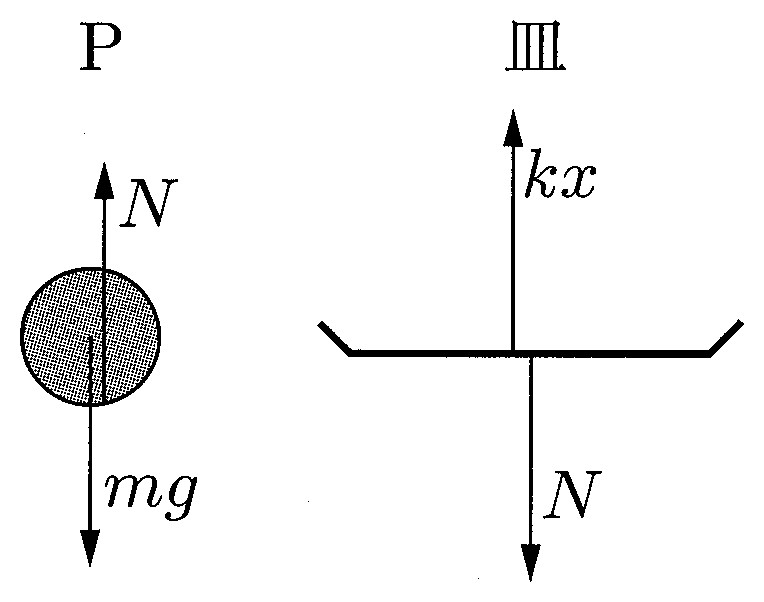
\includegraphics[keepaspectratio,width=60mm]{fig/ch3_p74_24.png}
\end{center}
\hspace{1zw}よって，
\begin{description}
\item[\MARU{1}] 皿が物体$\mathrm{P}$に及ぼす垂直抗力
\item[\MARU{2}] つり合い
\item[\MARU{3}] $mg\U{N}$
\item[\MARU{4}] 作用・反作用
\item[\MARU{5}] 物体$\mathrm{P}$が皿に及ぼす垂直抗力
\item[\MARU{6}] $kx=mg$
\item[\MARU{7}] $x=\dfrac{mg}{k}\U{m}$
\end{description}
\begin{chuu}
\hspace{1zw}\MARU{6}の立式の右辺にある$mg$は，物体$\mathrm{P}$に作用する重力ではなく，\MARU{5}の垂直抗力を表していることに注意せよ．この\MARU{5}の力は，\MARU{2}および\MARU{4}の事項より，大きさが$mg\U{N}$になっている．

% TODO: 原本では「バネばかり」表記（台ばかりの誤りと思われる）
\hspace{1zw}また，以上のことから分かるように，バネばかりは物体の質量そのものを計っているのではなく，バネばかりの皿に対して作用する力を計っている．すなわち，バネばかりの針が$m\U{kg}$を指している場合には，バネの皿に対して大きさ$mg\U{N}$の力が下向きに作用しているということを意味している．
\end{chuu}

\MonN{25}{力のつり合い}\par\nopagebreak
\begin{sisin}
\hspace{1zw}本問のような複雑な力のつり合いの問題でも，基本は\MARU{1}「作用している力の書き出し」，\MARU{2}「力のつり合いの式の立式」の二つの手順を踏むのみである．

\hspace{1zw}「なめらかな斜面」とは摩擦のない斜面のことを意味する．
\end{sisin}
\noindent{\gtfamily 【解答】}\par\nopagebreak
\hspace{1zw}糸が物体に及ぼす張力の大きさを$T\U{N}$，斜面が物体に及ぼす垂直抗力の大きさを$N\U{N}$とすれば，物体に働く力の作用図は図の通り．
\begin{center}
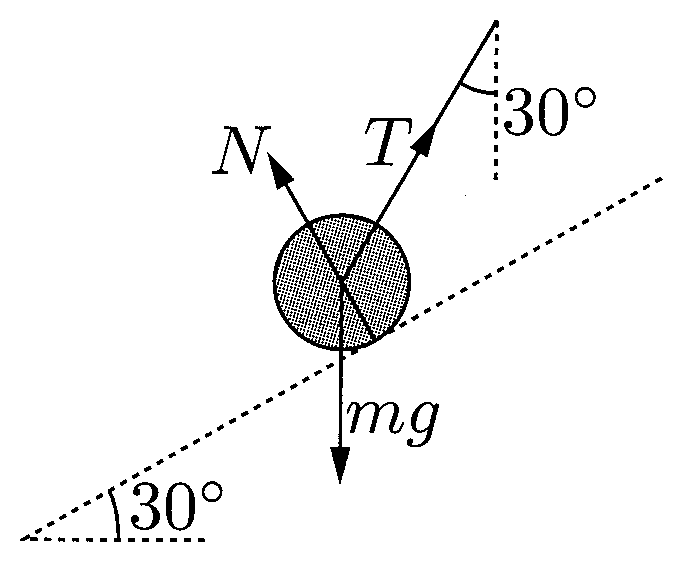
\includegraphics[keepaspectratio,width=50mm]{fig/ch3_p75_25.png}
\end{center}
\hspace{1zw}力のつり合いの式を立てると，
\[
\text{斜面に平行な方向：}\quad mg\sin30^\circ=T\cos30^\circ
\]
\[
\text{斜面に垂直な方向：}\quad N+T\sin30^\circ=mg\cos30^\circ
\]
よって，
\[
T=\dfrac{\sqrt3}{3}mg\U{N},\quad N=\dfrac{\sqrt3}{3}mg\U{N}\Ans
\]
\begin{bekkai}
\hspace{1zw}水平方向・鉛直方向に力を分解して考えてもよい．次のようになり，同じ答えが得られる．
\[
\text{水平方向：}\quad N\sin30^\circ=T\sin30^\circ
\]
\[
\text{鉛直方向：}\quad N\cos30^\circ+T\cos30^\circ=mg
\]
\end{bekkai}

\Rank{C問題}
\MonN{26}{弾性力}\par\nopagebreak
\begin{sisin}
\hspace{1zw}バネが物体に作用する力は，その伸び（もしくは縮み）によって決まる．バネの全長と伸びとを混同しないように注意せよ．
\end{sisin}
\noindent{\gtfamily 【解答】}\par\nopagebreak
\hspace{1zw}弾性定数を$k\U{N/m}$，重力加速度の大きさを$g\U{m/s^2}$とする．

\noindent\underline{物体$\mathrm{A}$について}\par
\hspace{1zw}このときのバネの全長は$\sqrt2\,l$であるから，自然長から$\left(\sqrt2-1\right)l$だけ伸びている．よって，物体$\mathrm{A}$にバネが作用する弾性力はフックの法則より$\left(\sqrt2-1\right)kl\U{N}$であり，物体$\mathrm{A}$に働く力の作用図は次図の通りとなる．
\begin{center}
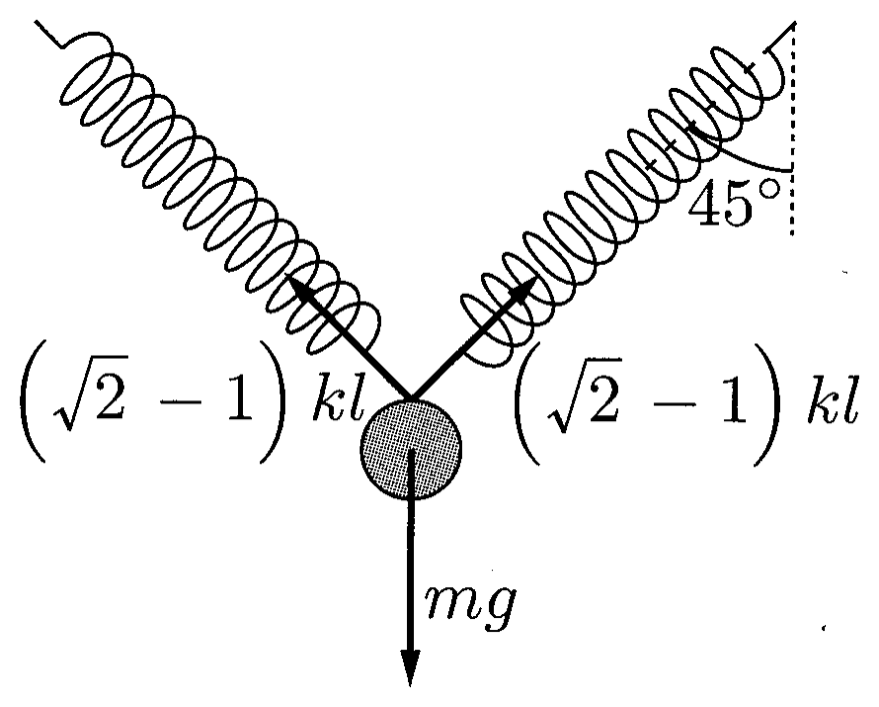
\includegraphics[keepaspectratio,width=62mm]{fig/ch3_p75_26.png}
\end{center}
\hspace{1zw}鉛直方向の力のつり合いについて，
\[
2\times\left(\sqrt2-1\right)kl\cos45^\circ=mg
\]
であるから，
\[
m=\dfrac{\left(2-\sqrt2\right)kl}{g}\U{kg}\Eq{1}
\]

\noindent\underline{物体$\mathrm{B}$について}\par
\hspace{1zw}同様に考えると，バネの全長は$2l\U{m}$なので，$\mathrm{B}$に作用する弾性力の大きさは$kl\U{N}$であり，鉛直方向の力のつり合いの式は，
\[
2\times kl\cos30^\circ=Mg
\]
よって，
\[
M=\dfrac{\sqrt3\,kl}{g}\U{kg}\Eq{2}
\]
\MARU{1}\MARU{2}より，
\[
\dfrac{m}{M}=\dfrac{2\sqrt3-\sqrt6}{3}\Ans
\]

\MonN{27}{斜面上での最大摩擦力}\par\nopagebreak
\begin{sisin}
\hspace{1zw}(1)については前出の問題と同じなのでよかろう．(2)についても基本的な考えは，力の作用図の作図，つり合いの式の立式である．問題なのは作用する静止摩擦力の向きである．この物体は重力の斜面方向分力$mg\sin\alpha$によって滑り出そうとするので，これを防ぐには静止摩擦力が上向きに作用すればよい．ところが$\alpha>\alpha_0$の場合には，物体が滑り出すのを防ぐために必要なだけの静止摩擦力を作用することができない．なるべく小さな力で物体が滑り出すのを防ぐためには，静止に必要な力を補うべく上向きに力を加えてやればよい．よって，作用している静止摩擦力は上向きと分かる．このような直観的な考え方が分かりにくい人は，静止摩擦力が下向きに作用する場合についても図を描いて立式し，考えてみよ．この場合，静止するのに必要な外力は，摩擦力が上向きに作用する場合に比べて大きくなることが計算によって示される．
\end{sisin}
\noindent{\gtfamily 【解答】}\par\nopagebreak
\hspace{1zw}物体に作用する垂直抗力の大きさを$N\U{N}$，静止摩擦力の大きさを$f\U{N}$とする．
\begin{komon}
\ko{1} 水平面との傾角が$\alpha_0$のとき，物体に働く力の作用図は次図の通り．
\begin{center}
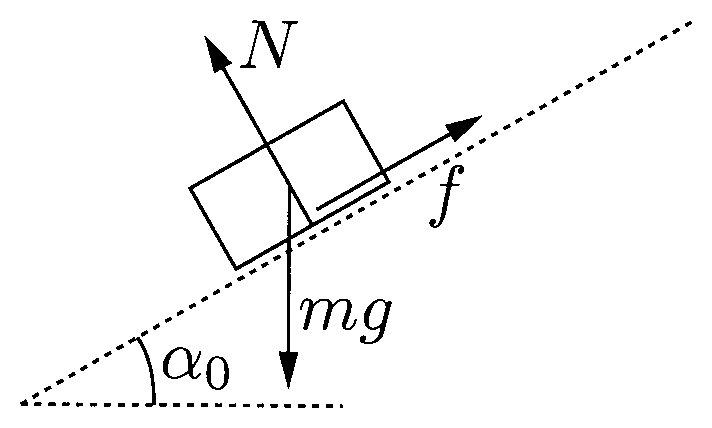
\includegraphics[keepaspectratio,width=55mm]{fig/ch3_p75_27a.png}
\end{center}

ここで，各方向の力のつり合いは，
\[
\text{斜面に平行な方向：}\quad mg\sin\alpha_0=f
\]
\[
\text{斜面に垂直な方向：}\quad N=mg\cos\alpha_0
\]
また，このとき板が物体に及ぼす静止摩擦力は最大摩擦力となっているので，
\[
f=\mu_0N
\]
以上より，
\[
\mu_0=\tan\alpha_0\Ans
\]
\ko{2} 水平面との傾角が$\alpha$のとき，物体がすべるのを防ぐために板と平行上向きに加える力の大きさを$f'$とする．このとき，物体に働く力は次図の通り．
\begin{center}
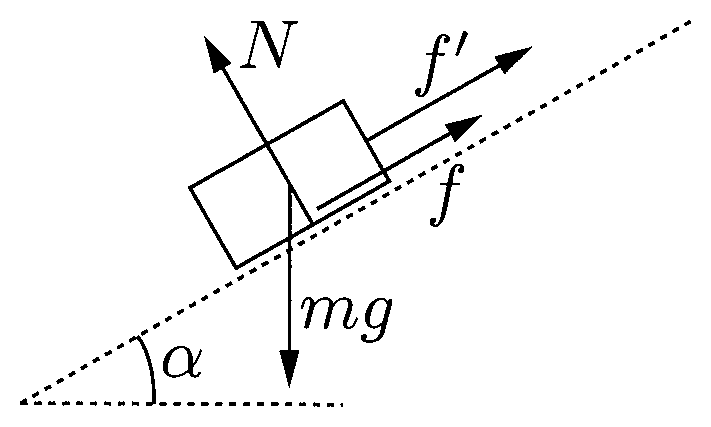
\includegraphics[keepaspectratio,width=55mm]{fig/ch3_p76_27b.png}
\end{center}

力のつり合いより，
\[
\text{斜面に平行な方向：}\quad mg\sin\alpha=f+f'
\]
% TODO: 原本ママ．「斜面に垂直な方向」の誤りと思われる
\[
\text{鉛直に垂直な方向：}\quad N=mg\cos\alpha
\]
物体が静止をしつづけるためには，作用している静止摩擦力が，最大摩擦力$\mu_0N$を越えなければよい．
\[
f\leqq\mu_0N
\]
以上の式を満たすような$f'$は，
\[
f'\geqq mg\left(\sin\alpha-\mu_0\cos\alpha\right)
\]
である．よって，加えるべき最小限の力の大きさは，これに(1)の答えを代入して
\[
mg\left(\sin\alpha-\tan\alpha_0\cos\alpha\right)\U{N}\Ans
\]
\end{komon}
\begin{itembox}[l]{【参考】}
\hspace{1zw}物体に加える力$f'$を大きくしていくと，いずれ物体は斜面にそって上向きに動き出す．動き始める瞬間の$f'$の大きさを求めてみよう．

\hspace{1zw}静止摩擦力の向きに注意すると，動き始める瞬間の力のつりあいの式は次のようになる．
\[
\text{斜面に平行な方向：}\quad mg\sin\alpha+f=f'
\]
% TODO: 原本ママ．「斜面に垂直な方向」の誤りと思われる
\[
\text{鉛直に垂直な方向：}\quad N=mg\cos\alpha
\]
これらと$f=\mu_0N$を連立すると，
\[
f'=mg\left(\sin\alpha+\tan\alpha_0\cos\alpha\right)
\]
が分かる．これが物体を上向きに動かすのに必要な最小の力であるから，物体を斜面上に静止させておくには，斜面にそって上向きに
\[
mg\left(\sin\alpha-\mu_0\cos\alpha\right)\leqq f'
\]
\[
\hspace{8zw}\leqq mg\left(\sin\alpha+\tan\alpha_0\cos\alpha\right)
\]
を満たす力$f'$を加えればよい．
\end{itembox}

\end{multicols}
